\chapter{PK9 --- Vận hành mô hình}
\begin{figure}[H]\centering
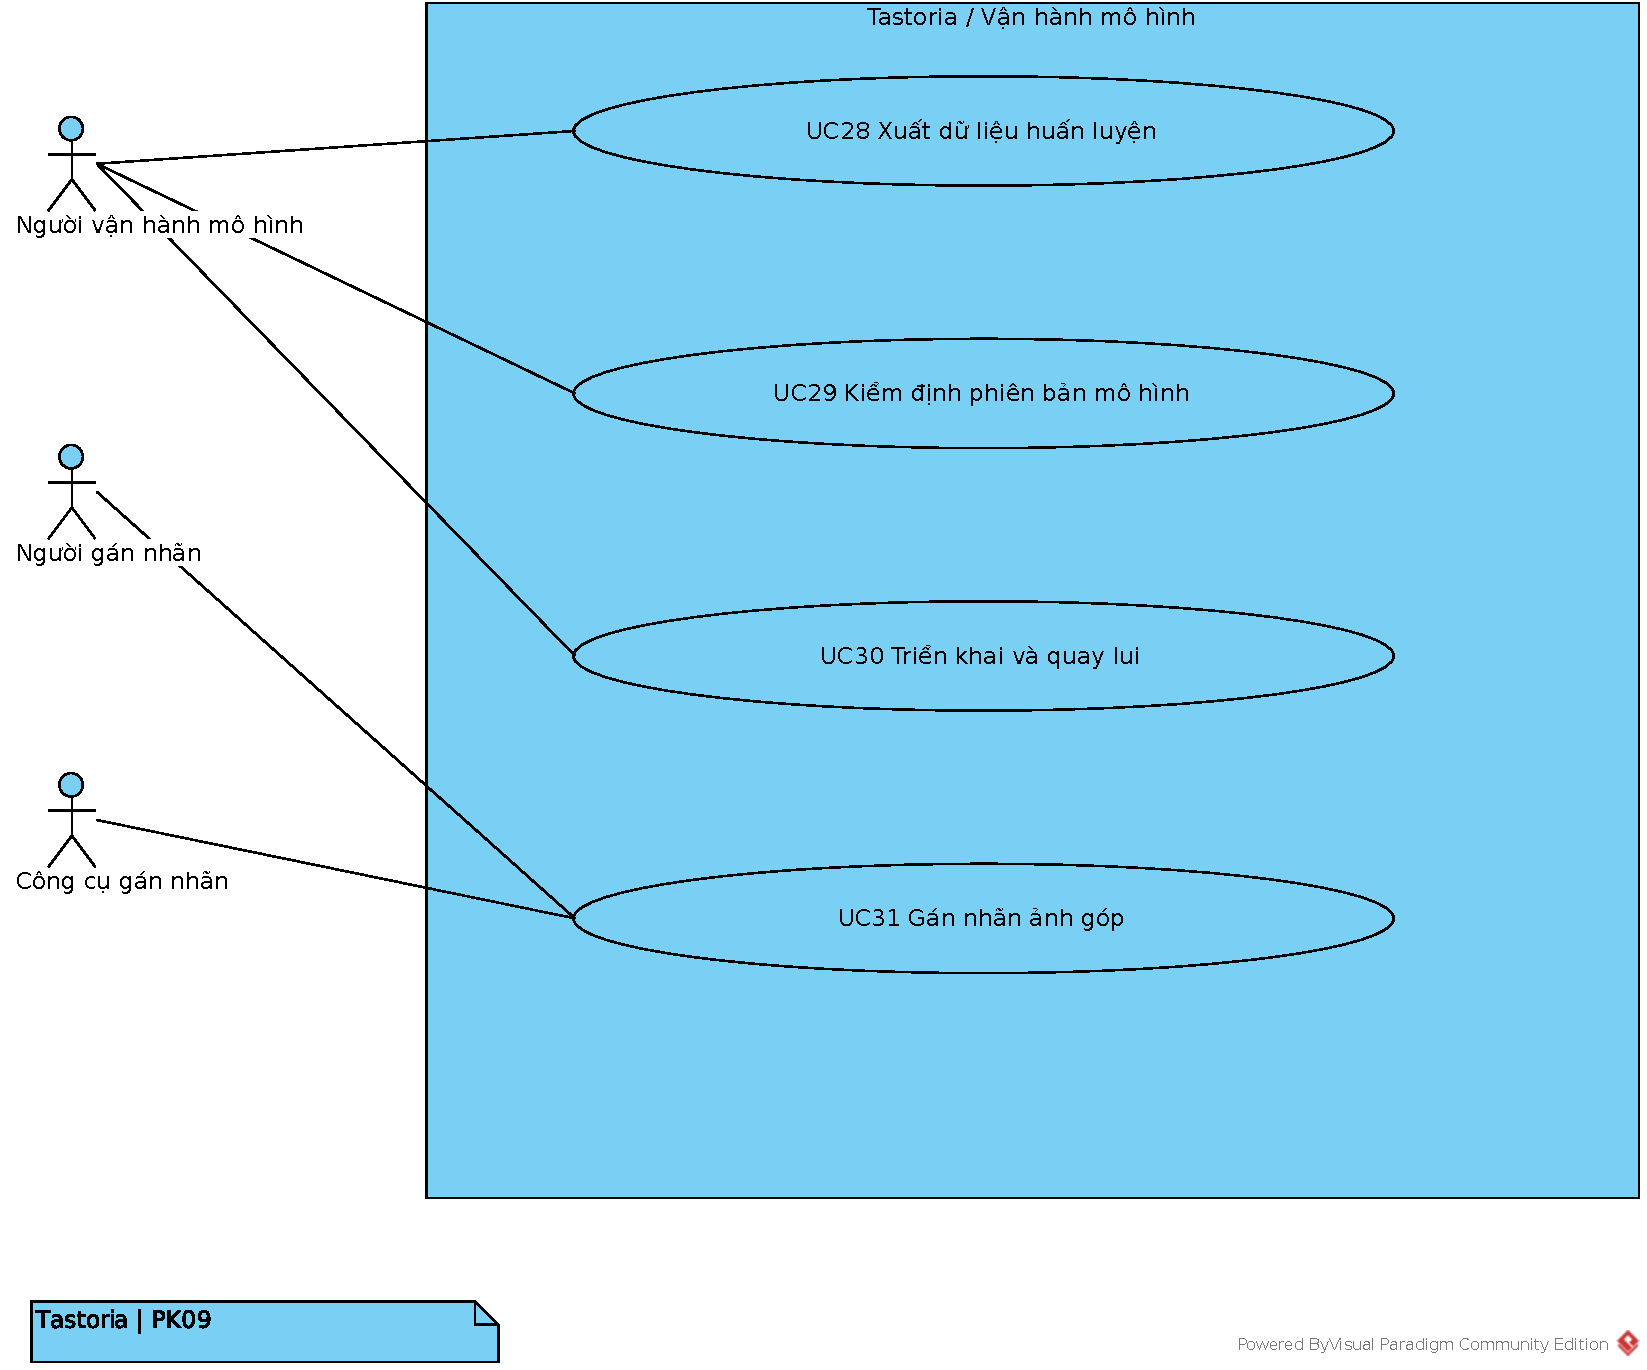
\includegraphics[width=0.96\linewidth,height=0.75\textheight,keepaspectratio]{assets/PK09.pdf}
\caption{PK09 --- Phân rã use case}\label{fig:Phu-luc-A-Use-Cases:9}
\end{figure}
\section{UC28 --- Xuất dữ liệu huấn luyện đã bí danh hoá}
\subsection{Mục tiêu trong ngữ cảnh}
Người vận hành mô hình (A06) xuất dữ liệu phát sinh trong app (tương tác với món, đổi món, sửa chip quét, ảnh góp) từ một mốc ngày để huấn luyện lại bộ xếp hạng, bộ phát hiện và bộ phân loại độ tươi trên máy lab L40S đặt tại Việt Nam. Bản xuất được \textbf{bí danh hoá} (HMAC-\allowbreak{}SHA256, khoá tách riêng) và vẫn được coi là dữ liệu cá nhân nhạy cảm; chỉ chứa dữ liệu mà chủ thể đang đồng ý cho đúng mục đích.

\subsection{Phạm vi và mức}
\begin{itemize}
\item Phạm vi: hệ thống Tastoria, module {\small\texttt{admin}} (CLI) gọi {\small\texttt{privacy}}, {\small\texttt{catalog}}, {\small\texttt{mlops}}; dữ liệu nguồn thuộc module {\small\texttt{events}} và {\small\texttt{scan}} (xem mục 16 về phụ thuộc).
\item Mức: mục tiêu người dùng, thao tác nhân sự qua CLI.
\end{itemize}
\subsection{Tác nhân và bên liên quan (quyền lợi)}
{\footnotesize\setlength{\tabcolsep}{0pt}
\begin{longtable}{@{}L{7.850cm}@{\hspace{3mm}}L{7.850cm}@{}}
\caption{Tác nhân và bên liên quan (quyền lợi)}\\
\toprule
\textbf{Bên} & \textbf{Quyền lợi} \\
\midrule\endfirsthead
\multicolumn{2}{l}{\small\itshape Bảng \thetable{} (tiếp theo)}\\
\toprule
\textbf{Bên} & \textbf{Quyền lợi} \\
\midrule\endhead
\bottomrule\endfoot
A06 Người vận hành mô hình & Bản xuất tái lập được (manifest, sha256), đủ trường để huấn luyện. \\ \addlinespace[3pt]
A02 Người dùng & Dữ liệu của mình chỉ ra khỏi DB khi đã đồng ý; rút đồng ý hay xoá tài khoản thì bị loại khỏi lần xuất kế tiếp và có danh sách bí danh cần xoá ở các bản cũ. \\ \addlinespace[3pt]
Bên kiểm soát dữ liệu & Không phát sinh chuyển dữ liệu xuyên biên giới (huấn luyện tại Việt Nam); có {\small\texttt{audit\_\allowbreak{}\allowbreak{}log}} mỗi lần xuất. \\ \addlinespace[3pt]
\end{longtable}}
\subsection{Tiền điều kiện}
\begin{enumerate}
\item A06 có quyền chạy lệnh trong container {\small\texttt{api}}.
\item Khoá HMAC xuất dữ liệu đã cấu hình, tách khỏi thư mục đích và khác khoá mã hoá cột.
\item Thư mục đích trên máy lab (Việt Nam) đã gắn vào container.
\end{enumerate}
\subsection{Đảm bảo tối thiểu}
Không có tệp xuất dở dang được coi là hợp lệ: tệp chỉ có tên cuối cùng sau khi manifest ghi xong. Không dòng nào chứa {\small\texttt{user\_\allowbreak{}\allowbreak{}id}}, email hay cột sức khoẻ. Mọi lần chạy ghi {\small\texttt{audit\_\allowbreak{}\allowbreak{}log}}.

\subsection{Đảm bảo khi thành công}
\begin{enumerate}
\item Thư mục xuất có các tệp dữ liệu và {\small\texttt{manifest}} (mốc {\small\texttt{since}}, thời điểm xuất, số dòng mỗi tệp, sha256 mỗi tệp, mã khoá HMAC, phiên bản mô hình đang chạy).
\item Mỗi {\small\texttt{user\_\allowbreak{}\allowbreak{}id}} được thay bằng bí danh HMAC-\allowbreak{}SHA256(khoá xuất, user\_\allowbreak{}id); thời điểm làm thô về ngày.
\item Có danh sách bí danh bị thu hồi (người rút đồng ý hoặc xoá tài khoản từ {\small\texttt{since}}) để xoá khỏi các bản xuất cũ.
\end{enumerate}
\subsection{Kích hoạt}
A06 chạy {\small\texttt{tastoria mlops export-\allowbreak{}training-\allowbreak{}data -\allowbreak{}-\allowbreak{}since <date>}} trước một vòng huấn luyện lại (dự kiến hằng tuần).

\subsection{Kịch bản chính}
\begin{enumerate}
\item A06 chạy {\small\texttt{tastoria mlops export-\allowbreak{}training-\allowbreak{}data -\allowbreak{}-\allowbreak{}since 2026-\allowbreak{}11-\allowbreak{}01}}.
\item Module {\small\texttt{admin}} kiểm tham số ngày và khoá HMAC.
\item Module {\small\texttt{admin}} gọi {\small\texttt{privacy.\allowbreak{}current\_\allowbreak{}\allowbreak{}consents()}} (đọc {\small\texttt{v\_\allowbreak{}\allowbreak{}current\_\allowbreak{}\allowbreak{}consents}}) lấy tập người đang đồng ý {\small\texttt{personalization}} và tập người đang đồng ý {\small\texttt{photo\_\allowbreak{}\allowbreak{}contribution}}; loại người có {\small\texttt{users.\allowbreak{}status = deletion\_\allowbreak{}\allowbreak{}requested}}.
\item Module {\small\texttt{admin}} đọc {\small\texttt{interactions}} (cùng {\small\texttt{meal\_\allowbreak{}\allowbreak{}plans}}, {\small\texttt{meal\_\allowbreak{}\allowbreak{}plan\_\allowbreak{}\allowbreak{}items}}) có {\small\texttt{occurred\_\allowbreak{}\allowbreak{}at \ensuremath{\geq} since}} của tập người đồng ý {\small\texttt{personalization}}; giữ {\small\texttt{recipe\_\allowbreak{}\allowbreak{}id}}, {\small\texttt{type}}, {\small\texttt{position}}, {\small\texttt{swap\_\allowbreak{}\allowbreak{}reason}}, {\small\texttt{ranker\_\allowbreak{}\allowbreak{}version\_\allowbreak{}\allowbreak{}id}}, {\small\texttt{propensity}}, ngày xảy ra.
\item Module {\small\texttt{admin}} đọc sửa chip ({\small\texttt{scan\_\allowbreak{}\allowbreak{}items}} có {\small\texttt{user\_\allowbreak{}\allowbreak{}action \ensuremath{\in} \{relabeled, deleted, edited\}}} hoặc {\small\texttt{origin = user\_\allowbreak{}\allowbreak{}added}}) và {\small\texttt{detections}} tương ứng, kèm {\small\texttt{scans.\allowbreak{}detector\_\allowbreak{}\allowbreak{}version\_\allowbreak{}\allowbreak{}id}}, của tập người đồng ý {\small\texttt{photo\_\allowbreak{}\allowbreak{}contribution}}.
\item Module {\small\texttt{admin}} lấy danh sách {\small\texttt{scan\_\allowbreak{}\allowbreak{}images}} có {\small\texttt{contributed = true}}, {\small\texttt{purged\_\allowbreak{}\allowbreak{}at}} NULL của tập người đồng ý {\small\texttt{photo\_\allowbreak{}\allowbreak{}contribution}}; xuất khoá lưu trữ tương đối (không kèm EXIF, ảnh đã mã hoá lại lúc tải lên).
\item Module {\small\texttt{admin}} thay mọi {\small\texttt{user\_\allowbreak{}\allowbreak{}id}} bằng bí danh HMAC-\allowbreak{}SHA256, làm thô thời điểm về ngày (Asia/\allowbreak{}Ho\_\allowbreak{}Chi\_\allowbreak{}Minh), bỏ id mâm/\allowbreak{}phiên/\allowbreak{}quét gốc bằng bí danh cùng khoá.
\item Module {\small\texttt{admin}} lập danh sách bí danh thu hồi từ {\small\texttt{consent\_\allowbreak{}\allowbreak{}events}} action {\small\texttt{withdraw}} và {\small\texttt{dsr\_\allowbreak{}\allowbreak{}requests}} loại {\small\texttt{delete}} hoàn tất từ {\small\texttt{since}}.
\item Module {\small\texttt{admin}} gọi {\small\texttt{catalog}} lấy bảng tra {\small\texttt{recipes}}, {\small\texttt{ingredients}}, {\small\texttt{vision\_\allowbreak{}\allowbreak{}classes}} cần cho huấn luyện; gọi {\small\texttt{mlops}} lấy phiên bản đang chạy.
\item Module {\small\texttt{admin}} ghi tệp tạm, tính sha256, ghi {\small\texttt{manifest}}, đổi tên tệp sang tên cuối.
\item Module {\small\texttt{admin}} gọi {\small\texttt{privacy.\allowbreak{}record\_\allowbreak{}\allowbreak{}audit()}} (action {\small\texttt{training\_\allowbreak{}\allowbreak{}export}}, purpose, số dòng); in đường dẫn và tóm tắt; thoát mã 0.
\end{enumerate}
\subsection{Mở rộng}
\begin{itemize}
\item \textbf{1a. {\small\texttt{-\allowbreak{}-\allowbreak{}since}} sai định dạng hoặc ở tương lai} (lỗi nhập): thoát mã \ensuremath{\neq} 0, không ghi tệp.
\item \textbf{2a. Thiếu khoá HMAC hoặc khoá nằm trong thư mục đích}: thoát mã \ensuremath{\neq} 0 (không bí danh hoá được thì không xuất).
\item \textbf{3a. Không ai đồng ý mục đích tương ứng} (thiếu đồng ý): tệp của mục đích đó rỗng nhưng vẫn có trong manifest với 0 dòng.
\item \textbf{3b. Người đã rút đồng ý sau khi sự kiện xảy ra}: không xuất (lọc theo đồng ý hiện hành, không theo đồng ý lúc ghi) --- BR-\allowbreak{}CONSENT-\allowbreak{}04.
\item \textbf{6a. Ảnh đã bị xoá theo BR-\allowbreak{}RETAIN-\allowbreak{}01} ({\small\texttt{purged\_\allowbreak{}\allowbreak{}at}} có giá trị): không xuất.
\item \textbf{10a. Thư mục đích đầy hoặc mất kết nối ổ} (lỗi hệ thống): xoá tệp tạm, không tạo manifest, thoát mã \ensuremath{\neq} 0, ghi {\small\texttt{audit\_\allowbreak{}\allowbreak{}log}} thất bại.
\item \textbf{10b. Chạy lại cùng {\small\texttt{-\allowbreak{}-\allowbreak{}since}} sau lỗi} (lũy đẳng): tạo thư mục xuất mới có tên theo thời điểm; dữ liệu cùng mốc cho cùng bí danh (HMAC tất định) nên ghép được với bản trước.
\item \textbf{*a. Quá thời gian}: không giới hạn cứng; A06 ngắt giữa chừng thì như 10a.
\item Quan hệ include/\allowbreak{}extend: model.yaml không khai báo include/\allowbreak{}extend cho UC28.
\end{itemize}
\subsection{Ghi chú đối chiếu của báo cáo}
Giữ phạm vi yêu cầu của đặc tả nguồn; cần kiểm thử theo môi trường và phiên bản thực tế trước khi ghi kết quả nghiệm thu.

\textbf{Nguồn:} {\small\texttt{Tastoria/\allowbreak{}\allowbreak{}docs/\allowbreak{}\allowbreak{}sad/\allowbreak{}\allowbreak{}use-\allowbreak{}cases/\allowbreak{}\allowbreak{}UC28.\allowbreak{}md}}. Mã nghiệp vụ: BR-\allowbreak{}CONSENT-\allowbreak{}03, BR-\allowbreak{}CONSENT-\allowbreak{}01, BR-\allowbreak{}CONSENT-\allowbreak{}04, BR-\allowbreak{}RETAIN-\allowbreak{}01, BR-\allowbreak{}DSR-\allowbreak{}01, BR-\allowbreak{}SWAP-\allowbreak{}01.

\textbf{Dữ liệu liên quan:} {\small\texttt{interactions}}, {\small\texttt{meal\_\allowbreak{}\allowbreak{}plans}}, {\small\texttt{meal\_\allowbreak{}\allowbreak{}plan\_\allowbreak{}\allowbreak{}items}}, {\small\texttt{scans}}, {\small\texttt{scan\_\allowbreak{}\allowbreak{}images}}, {\small\texttt{scan\_\allowbreak{}\allowbreak{}items}}, {\small\texttt{detections}}, {\small\texttt{v\_\allowbreak{}\allowbreak{}current\_\allowbreak{}\allowbreak{}consents}}, {\small\texttt{consent\_\allowbreak{}\allowbreak{}events}}, {\small\texttt{users}}, {\small\texttt{dsr\_\allowbreak{}\allowbreak{}requests}}, {\small\texttt{recipes}}, {\small\texttt{ingredients}}, {\small\texttt{vision\_\allowbreak{}\allowbreak{}classes}}, {\small\texttt{model\_\allowbreak{}\allowbreak{}versions}}, {\small\texttt{audit\_\allowbreak{}\allowbreak{}log}}.

\textbf{Điểm giao tiếp:} {\small\texttt{CLI tastoria mlops export-\allowbreak{}training-\allowbreak{}data -\allowbreak{}-\allowbreak{}since <date>}}.

\section{UC29 --- Đăng ký và kiểm định phiên bản mô hình}
\subsection{Mục tiêu trong ngữ cảnh}
Người vận hành mô hình (A06) đưa một tệp mô hình mới huấn luyện (bộ phát hiện, bộ phân loại độ tươi, bộ xếp hạng hoặc bộ thay thế) vào sổ phiên bản {\small\texttt{model\_\allowbreak{}\allowbreak{}versions}} kèm checksum, bản đồ lớp, phiên bản tiền xử lý và chỉ số; sau đó chạy cổng kiểm định để quyết định phiên bản có đủ điều kiện triển khai (UC30) hay không. Mục tiêu là chỉ phiên bản {\small\texttt{validated}} mới được triển khai, và mọi kết quả trên app truy được về phiên bản đã tạo ra nó.

\subsection{Phạm vi và mức}
\begin{itemize}
\item Phạm vi: hệ thống Tastoria, module {\small\texttt{admin}} (CLI, endpoint) gọi module {\small\texttt{mlops}} và {\small\texttt{catalog}}.
\item Mức: mục tiêu người dùng.
\end{itemize}
\subsection{Tác nhân và bên liên quan (quyền lợi)}
{\footnotesize\setlength{\tabcolsep}{0pt}
\begin{longtable}{@{}L{7.850cm}@{\hspace{3mm}}L{7.850cm}@{}}
\caption{Tác nhân và bên liên quan (quyền lợi)}\\
\toprule
\textbf{Bên} & \textbf{Quyền lợi} \\
\midrule\endfirsthead
\multicolumn{2}{l}{\small\itshape Bảng \thetable{} (tiếp theo)}\\
\toprule
\textbf{Bên} & \textbf{Quyền lợi} \\
\midrule\endhead
\bottomrule\endfoot
A06 Người vận hành mô hình & Đăng ký một lệnh; báo cáo kiểm định PASS/\allowbreak{}FAIL rõ ràng, lưu lại được. \\ \addlinespace[3pt]
A02 Người dùng & Không nhận mô hình kém hơn bản đang chạy. \\ \addlinespace[3pt]
Giám khảo các môn & Mỗi phiên bản có chỉ số, {\small\texttt{mlflow\_\allowbreak{}\allowbreak{}run\_\allowbreak{}\allowbreak{}id}}, báo cáo kiểm định để tái lập. \\ \addlinespace[3pt]
\end{longtable}}
\subsection{Tiền điều kiện}
\begin{enumerate}
\item A06 có quyền chạy lệnh trong container {\small\texttt{api}}; tài khoản {\small\texttt{role = ml\_\allowbreak{}\allowbreak{}operator}} để gọi {\small\texttt{GET /\allowbreak{}\allowbreak{}admin/\allowbreak{}\allowbreak{}models}}.
\item Tệp mô hình (ONNX, tệp vector NumPy hoặc LightGBM) và tệp chỉ số JSON đã được chép vào container.
\item Với bộ phát hiện và bộ độ tươi: {\small\texttt{vision\_\allowbreak{}\allowbreak{}classes}} đã có các lớp mô hình dùng.
\end{enumerate}
\subsection{Đảm bảo tối thiểu}
Không có phiên bản nào ở {\small\texttt{validated}} mà thiếu báo cáo kiểm định. Đăng ký thất bại không để lại bản ghi hay tệp mồ côi. Mọi lệnh ghi {\small\texttt{audit\_\allowbreak{}\allowbreak{}log}}.

\subsection{Đảm bảo khi thành công}
\begin{enumerate}
\item Sau {\small\texttt{register}}: một dòng {\small\texttt{model\_\allowbreak{}\allowbreak{}versions}} trạng thái {\small\texttt{candidate}}, tệp nằm trong thư mục {\small\texttt{models/\allowbreak{}\allowbreak{}}} với {\small\texttt{artifact\_\allowbreak{}\allowbreak{}key}}, {\small\texttt{sha256}} khớp tệp; {\small\texttt{model\_\allowbreak{}\allowbreak{}version\_\allowbreak{}\allowbreak{}classes}} đầy đủ nếu mô hình có lớp.
\item Sau {\small\texttt{gate}}: phiên bản chuyển {\small\texttt{validated}} (PASS) hoặc {\small\texttt{rejected}} (FAIL), {\small\texttt{gate\_\allowbreak{}\allowbreak{}report\_\allowbreak{}\allowbreak{}key}} trỏ báo cáo.
\end{enumerate}
\subsection{Kích hoạt}
A06 hoàn tất một lượt huấn luyện trên máy lab và muốn đưa mô hình vào hệ thống.

\subsection{Kịch bản chính}
\begin{enumerate}
\item A06 chạy {\small\texttt{tastoria mlops register detector .\allowbreak{}/\allowbreak{}\allowbreak{}yolo26n-\allowbreak{}v3.\allowbreak{}onnx -\allowbreak{}-\allowbreak{}metrics .\allowbreak{}/\allowbreak{}\allowbreak{}metrics.\allowbreak{}json}} (kèm phiên bản, phiên bản tiền xử lý, bản đồ lớp, {\small\texttt{mlflow\_\allowbreak{}\allowbreak{}run\_\allowbreak{}\allowbreak{}id}}).
\item Module {\small\texttt{admin}} đọc tệp chỉ số JSON, gọi {\small\texttt{mlops.\allowbreak{}register\_\allowbreak{}\allowbreak{}version()}}.
\item Module {\small\texttt{mlops}} tính sha256 của tệp, chép tệp vào {\small\texttt{models/\allowbreak{}\allowbreak{}}} qua lưu tệp của {\small\texttt{core}}, kiểm {\small\texttt{name \ensuremath{\in} \{detector, freshness, ranker, substitution\}}}, kiểm (name, version) chưa tồn tại.
\item Với {\small\texttt{detector}} và {\small\texttt{freshness}}, module {\small\texttt{mlops}} gọi {\small\texttt{catalog}} kiểm mỗi {\small\texttt{vision\_\allowbreak{}\allowbreak{}class\_\allowbreak{}\allowbreak{}id}} trong bản đồ lớp tồn tại, {\small\texttt{class\_\allowbreak{}\allowbreak{}index}} liên tục từ 0; với {\small\texttt{freshness}}, lớp được liệt kê phải có {\small\texttt{has\_\allowbreak{}\allowbreak{}freshness\_\allowbreak{}\allowbreak{}model = true}}.
\item Module {\small\texttt{mlops}} ghi {\small\texttt{model\_\allowbreak{}\allowbreak{}versions}} ({\small\texttt{status = candidate}}) và {\small\texttt{model\_\allowbreak{}\allowbreak{}version\_\allowbreak{}\allowbreak{}classes}} trong một Unit of Work; module {\small\texttt{admin}} ghi {\small\texttt{audit\_\allowbreak{}\allowbreak{}log}} (action {\small\texttt{model.\allowbreak{}register}}).
\item A06 chạy {\small\texttt{tastoria mlops gate detector v3}}.
\item Module {\small\texttt{admin}} gọi {\small\texttt{mlops.\allowbreak{}run\_\allowbreak{}\allowbreak{}gate()}}; module {\small\texttt{mlops}} đọc {\small\texttt{model\_\allowbreak{}\allowbreak{}deployments}} lấy bản đang chạy cùng {\small\texttt{name}} làm mốc so.
\item Module {\small\texttt{mlops}} đánh giá phiên bản ứng viên và bản đang chạy trên tập kiểm tra đóng băng (danh sách id cố định, có sha256), tính chỉ số chính và khoảng tin cậy bootstrap của hiệu (ứng viên - đang chạy).
\item Module {\small\texttt{mlops}} kết luận PASS nếu cận dưới khoảng tin cậy của hiệu \ensuremath{\geq} -\ensuremath{\delta} (biên không kém chọn trước), ngược lại FAIL; ghi báo cáo vào {\small\texttt{models/\allowbreak{}\allowbreak{}}}, đặt {\small\texttt{gate\_\allowbreak{}\allowbreak{}report\_\allowbreak{}\allowbreak{}key}}, chuyển {\small\texttt{status}} sang {\small\texttt{validated}} hoặc {\small\texttt{rejected}}.
\item Module {\small\texttt{admin}} ghi {\small\texttt{audit\_\allowbreak{}\allowbreak{}log}} (action {\small\texttt{model.\allowbreak{}gate}}, kết quả) và in tóm tắt; thoát mã 0 khi PASS, mã khác 0 khi FAIL.
\item A06 xem danh sách phiên bản, trạng thái và con trỏ triển khai qua {\small\texttt{GET /\allowbreak{}\allowbreak{}admin/\allowbreak{}\allowbreak{}models}}.
\end{enumerate}
\subsection{Mở rộng}
\begin{itemize}
\item \textbf{1a. Tệp mô hình hoặc tệp chỉ số không đọc được, JSON sai} (lỗi nhập): thoát mã \ensuremath{\neq} 0, không ghi gì.
\item \textbf{3a. (name, version) đã tồn tại với cùng sha256} (gửi lại lũy đẳng): trả phiên bản đã có, không tạo bản ghi mới, thoát mã 0.
\item \textbf{3b. (name, version) đã tồn tại với sha256 khác}: lỗi chặn, thoát mã \ensuremath{\neq} 0 (không ghi đè phiên bản).
\item \textbf{4a. Bản đồ lớp trỏ lớp không tồn tại hoặc {\small\texttt{class\_\allowbreak{}\allowbreak{}index}} bị hở}: lỗi chặn; xoá tệp vừa chép; không ghi bản ghi.
\item \textbf{5a. Lỗi hệ thống khi ghi DB}: rollback; tệp vừa chép bị xoá; chạy lại an toàn.
\item \textbf{6a. Phiên bản không ở {\small\texttt{candidate}}} (đã {\small\texttt{validated}}/\allowbreak{}{\small\texttt{rejected}}): lỗi 409 tương đương, thoát mã \ensuremath{\neq} 0; báo cáo cũ giữ nguyên.
\item \textbf{7a. Chưa có bản đang chạy cho {\small\texttt{name}} này} (lần triển khai đầu): cổng so với ngưỡng tuyệt đối đặt trước trong tệp cấu hình cổng (xem mục 16); thiếu ngưỡng thì FAIL với lý do "không có mốc so".
\item \textbf{8a. Tập kiểm tra đóng băng có sha256 khác giá trị đã khoá}: FAIL với lý do "tập kiểm tra bị đổi".
\item \textbf{8b. Bộ độ tươi không có ngưỡng nhãn đã khoá trên validation} (BR-\allowbreak{}FRESH-\allowbreak{}04) hoặc thiếu hệ số hiệu chỉnh nhiệt độ (BR-\allowbreak{}FRESH-\allowbreak{}02): FAIL.
\item \textbf{8c. Quá thời gian hoặc hết bộ nhớ khi đánh giá}: phiên bản giữ {\small\texttt{candidate}}; thoát mã \ensuremath{\neq} 0; chạy lại được.
\item \textbf{11a. Gọi {\small\texttt{GET /\allowbreak{}\allowbreak{}admin/\allowbreak{}\allowbreak{}models}} không có vai trò {\small\texttt{ml\_\allowbreak{}\allowbreak{}operator}}}: 403.
\item Quan hệ include/\allowbreak{}extend: model.yaml không khai báo include/\allowbreak{}extend cho UC29; UC30 chỉ nhận phiên bản {\small\texttt{validated}} do UC29 tạo.
\end{itemize}
\subsection{Ghi chú đối chiếu của báo cáo}
Tiêu chí chất lượng trong đặc tả là cổng nghiệm thu mong muốn; không coi đã đạt nếu chưa có artifact và báo cáo đánh giá đúng phiên bản.

\textbf{Nguồn:} {\small\texttt{Tastoria/\allowbreak{}\allowbreak{}docs/\allowbreak{}\allowbreak{}sad/\allowbreak{}\allowbreak{}use-\allowbreak{}cases/\allowbreak{}\allowbreak{}UC29.\allowbreak{}md}}. Mã nghiệp vụ: BR-\allowbreak{}FRESH-\allowbreak{}02, BR-\allowbreak{}FRESH-\allowbreak{}04.

\textbf{Dữ liệu liên quan:} {\small\texttt{model\_\allowbreak{}\allowbreak{}versions}}, {\small\texttt{model\_\allowbreak{}\allowbreak{}version\_\allowbreak{}\allowbreak{}classes}}, {\small\texttt{model\_\allowbreak{}\allowbreak{}deployments}}, {\small\texttt{vision\_\allowbreak{}\allowbreak{}classes}}, {\small\texttt{audit\_\allowbreak{}\allowbreak{}log}}.

\textbf{Điểm giao tiếp:} {\small\texttt{CLI tastoria mlops register <name> <artifact> -\allowbreak{}-\allowbreak{}metrics <json>}}; {\small\texttt{CLI tastoria mlops gate <name> <version>}}; {\small\texttt{GET /\allowbreak{}\allowbreak{}admin/\allowbreak{}\allowbreak{}models}}.

\section{UC30 --- Triển khai và quay lui phiên bản mô hình}
\subsection{Mục tiêu trong ngữ cảnh}
Người vận hành mô hình (A06) đưa một phiên bản đã {\small\texttt{validated}} (UC29) vào phục vụ bằng cách đổi con trỏ {\small\texttt{model\_\allowbreak{}\allowbreak{}deployments}} rồi khởi động lại {\small\texttt{api}} và {\small\texttt{worker}}; khi bản mới có vấn đề, quay lui về bản trước trong < 5 phút (spec \S{}8). {\small\texttt{model\_\allowbreak{}\allowbreak{}deployments}} là nguồn sự thật duy nhất về bản đang chạy.

\subsection{Phạm vi và mức}
\begin{itemize}
\item Phạm vi: hệ thống Tastoria, module {\small\texttt{admin}} (CLI) gọi {\small\texttt{mlops}}; tiến trình {\small\texttt{api}} và {\small\texttt{worker}} nạp mô hình qua {\small\texttt{mlops}} khi khởi động.
\item Mức: mục tiêu người dùng.
\end{itemize}
\subsection{Tác nhân và bên liên quan (quyền lợi)}
{\footnotesize\setlength{\tabcolsep}{0pt}
\begin{longtable}{@{}L{7.850cm}@{\hspace{3mm}}L{7.850cm}@{}}
\caption{Tác nhân và bên liên quan (quyền lợi)}\\
\toprule
\textbf{Bên} & \textbf{Quyền lợi} \\
\midrule\endfirsthead
\multicolumn{2}{l}{\small\itshape Bảng \thetable{} (tiếp theo)}\\
\toprule
\textbf{Bên} & \textbf{Quyền lợi} \\
\midrule\endhead
\bottomrule\endfoot
A06 Người vận hành mô hình & Đổi bản một lệnh; quay lui nhanh; biết chắc tiến trình nạp đúng tệp. \\ \addlinespace[3pt]
A02 Người dùng & Quét và mâm không bị gián đoạn lâu; không chạy mô hình bị sửa tệp. \\ \addlinespace[3pt]
Nhóm đồ án & Mỗi lần quét/\allowbreak{}mâm ghi phiên bản đã dùng nên đối chiếu được trước và sau triển khai. \\ \addlinespace[3pt]
\end{longtable}}
\subsection{Tiền điều kiện}
\begin{enumerate}
\item A06 có quyền chạy lệnh trong container {\small\texttt{api}} và quyền {\small\texttt{docker compose restart}} trên máy chủ.
\item Phiên bản cần triển khai có {\small\texttt{status = validated}} (với {\small\texttt{deploy}}); {\small\texttt{model\_\allowbreak{}\allowbreak{}deployments}} có {\small\texttt{previous\_\allowbreak{}\allowbreak{}version\_\allowbreak{}\allowbreak{}id}} (với {\small\texttt{rollback}}).
\end{enumerate}
\subsection{Đảm bảo tối thiểu}
Con trỏ luôn trỏ một phiên bản có tệp tồn tại và sha256 khớp; tiến trình không phục vụ với mô hình có sha256 sai. Mỗi lần đổi con trỏ ghi {\small\texttt{audit\_\allowbreak{}\allowbreak{}log}}.

\subsection{Đảm bảo khi thành công}
\begin{enumerate}
\item {\small\texttt{model\_\allowbreak{}\allowbreak{}deployments}} của {\small\texttt{name}}: {\small\texttt{active\_\allowbreak{}\allowbreak{}version\_\allowbreak{}\allowbreak{}id}} = bản mới, {\small\texttt{previous\_\allowbreak{}\allowbreak{}version\_\allowbreak{}\allowbreak{}id}} = bản cũ, {\small\texttt{switched\_\allowbreak{}\allowbreak{}at}}, {\small\texttt{switched\_\allowbreak{}\allowbreak{}by}}.
\item Sau khởi động lại, {\small\texttt{api}} và {\small\texttt{worker}} nạp đúng bản; {\small\texttt{GET /\allowbreak{}\allowbreak{}readyz}} trả sẵn sàng.
\item Quét mới ghi {\small\texttt{scans.\allowbreak{}detector\_\allowbreak{}\allowbreak{}version\_\allowbreak{}\allowbreak{}id}}/\allowbreak{}{\small\texttt{classifier\_\allowbreak{}\allowbreak{}version\_\allowbreak{}\allowbreak{}id}}, mâm mới ghi {\small\texttt{meal\_\allowbreak{}\allowbreak{}plans.\allowbreak{}ranker\_\allowbreak{}\allowbreak{}version\_\allowbreak{}\allowbreak{}id}} bằng bản mới.
\end{enumerate}
\subsection{Kích hoạt}
A06 quyết định đưa bản {\small\texttt{validated}} vào phục vụ, hoặc phát hiện bản đang chạy lỗi (độ trễ, tỉ lệ sửa chip tăng, lỗi nạp) và cần quay lui.

\subsection{Kịch bản chính}
\begin{enumerate}
\item A06 chạy {\small\texttt{tastoria mlops deploy detector v3}}.
\item Module {\small\texttt{admin}} gọi {\small\texttt{mlops.\allowbreak{}deploy()}}; module {\small\texttt{mlops}} kiểm phiên bản tồn tại, {\small\texttt{status = validated}}, tệp tại {\small\texttt{artifact\_\allowbreak{}\allowbreak{}key}} tồn tại và sha256 khớp.
\item Module {\small\texttt{mlops}} cập nhật {\small\texttt{model\_\allowbreak{}\allowbreak{}deployments}} trong một Unit of Work: {\small\texttt{previous\_\allowbreak{}\allowbreak{}version\_\allowbreak{}\allowbreak{}id}} \ensuremath{\leftarrow} bản đang chạy, {\small\texttt{active\_\allowbreak{}\allowbreak{}version\_\allowbreak{}\allowbreak{}id}} \ensuremath{\leftarrow} bản mới, {\small\texttt{switched\_\allowbreak{}\allowbreak{}at}} \ensuremath{\leftarrow} now, {\small\texttt{switched\_\allowbreak{}\allowbreak{}by}} \ensuremath{\leftarrow} tài khoản nhân sự; ghi {\small\texttt{audit\_\allowbreak{}\allowbreak{}log}} (action {\small\texttt{model.\allowbreak{}deploy}}).
\item Module {\small\texttt{admin}} in hướng dẫn khởi động lại; A06 chạy {\small\texttt{docker compose restart api worker}}.
\item Khi khởi động, tiến trình {\small\texttt{api}} và {\small\texttt{worker}} gọi {\small\texttt{mlops.\allowbreak{}load\_\allowbreak{}\allowbreak{}active()}}: đọc con trỏ, kiểm sha256 tệp, nạp mô hình (bộ phát hiện, bộ độ tươi trong {\small\texttt{worker}} với {\small\texttt{intra\_\allowbreak{}\allowbreak{}op\_\allowbreak{}\allowbreak{}num\_\allowbreak{}\allowbreak{}threads = 2}}; bộ xếp hạng dạng vector NumPy trong {\small\texttt{api}}) cùng bản đồ lớp {\small\texttt{model\_\allowbreak{}\allowbreak{}version\_\allowbreak{}\allowbreak{}classes}}.
\item {\small\texttt{GET /\allowbreak{}\allowbreak{}readyz}} trả sẵn sàng sau khi mọi mô hình cần thiết đã nạp.
\item A06 kiểm qua {\small\texttt{GET /\allowbreak{}\allowbreak{}admin/\allowbreak{}\allowbreak{}models}} thấy bản mới là {\small\texttt{active}}.
\item (Quay lui) A06 chạy {\small\texttt{tastoria mlops rollback detector}}; module {\small\texttt{mlops}} hoán đổi {\small\texttt{active\_\allowbreak{}\allowbreak{}version\_\allowbreak{}\allowbreak{}id}} và {\small\texttt{previous\_\allowbreak{}\allowbreak{}version\_\allowbreak{}\allowbreak{}id}}, ghi {\small\texttt{audit\_\allowbreak{}\allowbreak{}log}} (action {\small\texttt{model.\allowbreak{}rollback}}); A06 khởi động lại như bước 4--6.
\end{enumerate}
\subsection{Mở rộng}
\begin{itemize}
\item \textbf{2a. Phiên bản không tồn tại} (lỗi nhập): thoát mã \ensuremath{\neq} 0, con trỏ không đổi.
\item \textbf{2b. Phiên bản không ở {\small\texttt{validated}}} ({\small\texttt{candidate}}, {\small\texttt{rejected}}, {\small\texttt{retired}}): từ chối; con trỏ không đổi.
\item \textbf{2c. Tệp thiếu hoặc sha256 không khớp}: từ chối; ghi {\small\texttt{audit\_\allowbreak{}\allowbreak{}log}} lỗi toàn vẹn.
\item \textbf{2d. Phiên bản đã là bản đang chạy} (gửi lại lũy đẳng): không đổi con trỏ, không ghi đè {\small\texttt{previous\_\allowbreak{}\allowbreak{}version\_\allowbreak{}\allowbreak{}id}}; thoát mã 0 với thông báo "đã đang chạy".
\item \textbf{5a. sha256 tệp lúc nạp không khớp} (tệp bị sửa sau khi triển khai): tiến trình không nạp, {\small\texttt{GET /\allowbreak{}\allowbreak{}readyz}} trả chưa sẵn sàng với mã lỗi; A06 quay lui (bước 8).
\item \textbf{5b. Nạp mô hình lỗi hoặc quá thời gian} (hết bộ nhớ trong {\small\texttt{-\allowbreak{}-\allowbreak{}memory=4g}}): như 5a.
\item \textbf{5c. Job quét đang chạy lúc khởi động lại {\small\texttt{worker}}}: job bị ngắt được sweeper (UC34) đưa lại hàng đợi; quét ghi phiên bản của lần chạy thành công.
\item \textbf{8a. Không có {\small\texttt{previous\_\allowbreak{}\allowbreak{}version\_\allowbreak{}\allowbreak{}id}}}: rollback từ chối, thoát mã \ensuremath{\neq} 0.
\item \textbf{8b. Bản trước đã chuyển {\small\texttt{retired}} hoặc tệp đã xoá}: rollback từ chối; A06 triển khai một bản {\small\texttt{validated}} khác bằng {\small\texttt{deploy}}.
\item \textbf{*a. Quá thời gian quay lui}: mục tiêu từ lệnh rollback đến {\small\texttt{GET /\allowbreak{}\allowbreak{}readyz}} sẵn sàng < 5 phút; vượt thì ghi vào báo cáo diễn tập.
\item \textbf{*b. Lỗi hệ thống khi ghi con trỏ}: rollback giao dịch; con trỏ giữ bản cũ.
\item Quan hệ include/\allowbreak{}extend: model.yaml không khai báo include/\allowbreak{}extend cho UC30; phụ thuộc kết quả của UC29.
\end{itemize}
\subsection{Ghi chú đối chiếu của báo cáo}
Phân biệt có quy trình đăng ký/\allowbreak{}triển khai với chất lượng mô hình. Không kết luận mô hình đang triển khai đạt mọi NFR chỉ từ trạng thái deployed.

\textbf{Nguồn:} {\small\texttt{Tastoria/\allowbreak{}\allowbreak{}docs/\allowbreak{}\allowbreak{}sad/\allowbreak{}\allowbreak{}use-\allowbreak{}cases/\allowbreak{}\allowbreak{}UC30.\allowbreak{}md}}. Mã nghiệp vụ: .

\textbf{Dữ liệu liên quan:} {\small\texttt{model\_\allowbreak{}\allowbreak{}deployments}}, {\small\texttt{model\_\allowbreak{}\allowbreak{}versions}}, {\small\texttt{model\_\allowbreak{}\allowbreak{}version\_\allowbreak{}\allowbreak{}classes}}, {\small\texttt{scans}}, {\small\texttt{meal\_\allowbreak{}\allowbreak{}plans}}, {\small\texttt{interactions}}, {\small\texttt{audit\_\allowbreak{}\allowbreak{}log}}.

\textbf{Điểm giao tiếp:} {\small\texttt{CLI tastoria mlops deploy <name> <version>}}; {\small\texttt{CLI tastoria mlops rollback <name>}}; {\small\texttt{GET /\allowbreak{}\allowbreak{}admin/\allowbreak{}\allowbreak{}models}}.

\section{UC31 --- Gán nhãn ảnh góp}
\subsection{Mục tiêu trong ngữ cảnh}
Người gán nhãn (A07) gán khung và tên lớp (và nhãn độ tươi khi có) cho ảnh quét mà người dùng đã đồng ý góp, để bổ sung tập huấn luyện. Hệ thống đẩy ảnh đủ điều kiện sang Công cụ gán nhãn (A10, Label Studio tự host trên máy lab), rồi kéo nhãn đã gán về. Ảnh được chọn ưu tiên theo tín hiệu học chủ động (chip bị người dùng sửa). Nhãn từ người dùng sửa chip không được coi là nhãn khung.

\subsection{Phạm vi và mức}
\begin{itemize}
\item Phạm vi: hệ thống Tastoria, module {\small\texttt{admin}} (CLI) gọi {\small\texttt{privacy}}, {\small\texttt{catalog}}; dữ liệu ảnh thuộc module {\small\texttt{scan}} (xem mục 16); A10 là hệ thống ngoài.
\item Mức: mục tiêu người dùng.
\end{itemize}
\subsection{Tác nhân và bên liên quan (quyền lợi)}
{\footnotesize\setlength{\tabcolsep}{0pt}
\begin{longtable}{@{}L{7.850cm}@{\hspace{3mm}}L{7.850cm}@{}}
\caption{Tác nhân và bên liên quan (quyền lợi)}\\
\toprule
\textbf{Bên} & \textbf{Quyền lợi} \\
\midrule\endfirsthead
\multicolumn{2}{l}{\small\itshape Bảng \thetable{} (tiếp theo)}\\
\toprule
\textbf{Bên} & \textbf{Quyền lợi} \\
\midrule\endhead
\bottomrule\endfoot
A07 Người gán nhãn & Có hàng ảnh cần gán, không trùng; danh sách lớp đúng {\small\texttt{vision\_\allowbreak{}\allowbreak{}classes}}. \\ \addlinespace[3pt]
A10 Công cụ gán nhãn & Nhận tác vụ có id ổn định, ảnh không metadata. \\ \addlinespace[3pt]
A02 Người dùng & Chỉ ảnh đã đồng ý góp mới ra khỏi kho; rút đồng ý thì ảnh bị gỡ khỏi công cụ gán nhãn. \\ \addlinespace[3pt]
A06 Người vận hành mô hình & Nhãn hợp lệ (toạ độ, lớp) để huấn luyện. \\ \addlinespace[3pt]
\end{longtable}}
\subsection{Tiền điều kiện}
\begin{enumerate}
\item Người chạy lệnh (A07 hoặc A06 thay mặt) có quyền chạy lệnh trong container {\small\texttt{api}}.
\item Label Studio chạy trên máy lab, có dự án với cấu hình lớp khớp {\small\texttt{vision\_\allowbreak{}\allowbreak{}classes}}, token truy cập đã cấu hình.
\end{enumerate}
\subsection{Đảm bảo tối thiểu}
Không ảnh nào của người không có đồng ý {\small\texttt{photo\_\allowbreak{}\allowbreak{}contribution}} hiện hành nằm trong công cụ gán nhãn sau lần {\small\texttt{push}} kế tiếp. Nhãn sai định dạng không được nhận. Mọi lần chạy ghi {\small\texttt{audit\_\allowbreak{}\allowbreak{}log}}.

\subsection{Đảm bảo khi thành công}
\begin{enumerate}
\item Sau {\small\texttt{push}}: mỗi ảnh đủ điều kiện có đúng một tác vụ trong Label Studio, gắn id {\small\texttt{scan\_\allowbreak{}\allowbreak{}images.\allowbreak{}id}}; ảnh hết điều kiện bị gỡ.
\item Sau {\small\texttt{pull}}: nhãn hoàn tất được lưu thành tập dữ liệu có phiên bản (tệp + sha256) trong vùng {\small\texttt{contrib/\allowbreak{}\allowbreak{}}}.
\end{enumerate}
\subsection{Kích hoạt}
Có thêm ảnh góp mới (định kỳ hằng tuần) hoặc A07 hoàn tất một đợt gán.

\subsection{Kịch bản chính}
\begin{enumerate}
\item A07 chạy {\small\texttt{tastoria labeling push}}.
\item Module {\small\texttt{admin}} gọi {\small\texttt{privacy.\allowbreak{}current\_\allowbreak{}\allowbreak{}consents()}} lấy người đang đồng ý {\small\texttt{photo\_\allowbreak{}\allowbreak{}contribution}}.
\item Module {\small\texttt{admin}} chọn {\small\texttt{scan\_\allowbreak{}\allowbreak{}images}} có {\small\texttt{contributed = true}}, {\small\texttt{purged\_\allowbreak{}\allowbreak{}at}} NULL, thuộc người đã đồng ý; sắp ưu tiên ảnh có chip bị sửa ({\small\texttt{scan\_\allowbreak{}\allowbreak{}items.\allowbreak{}user\_\allowbreak{}\allowbreak{}action \ensuremath{\in} \{relabeled, deleted, edited\}}} hoặc {\small\texttt{origin = user\_\allowbreak{}\allowbreak{}added}}).
\item Module {\small\texttt{admin}} gửi sang A10 các tác vụ mới (ảnh, id {\small\texttt{scan\_\allowbreak{}\allowbreak{}images.\allowbreak{}id}}, khung dự đoán của mô hình từ {\small\texttt{detections}} làm gợi ý), không gửi {\small\texttt{user\_\allowbreak{}\allowbreak{}id}} hay thông tin tài khoản.
\item Module {\small\texttt{admin}} gỡ khỏi A10 các tác vụ có ảnh không còn đủ điều kiện (rút đồng ý, tài khoản xoá, ảnh đã xoá).
\item Module {\small\texttt{admin}} ghi {\small\texttt{audit\_\allowbreak{}\allowbreak{}log}} (action {\small\texttt{labeling.\allowbreak{}push}}, số tác vụ thêm/\allowbreak{}gỡ); in tóm tắt.
\item A07 gán khung và lớp trong Label Studio (ngoài hệ thống).
\item A07 chạy {\small\texttt{tastoria labeling pull}}.
\item Module {\small\texttt{admin}} lấy nhãn đã hoàn tất từ A10, kiểm từng khung: toạ độ chuẩn hoá thoả 0 \ensuremath{\leq} x1 < x2 \ensuremath{\leq} 1, 0 \ensuremath{\leq} y1 < y2 \ensuremath{\leq} 1; lớp có trong {\small\texttt{vision\_\allowbreak{}\allowbreak{}classes}}; ảnh vẫn đủ điều kiện.
\item Module {\small\texttt{admin}} ghi tập nhãn hợp lệ thành tệp có phiên bản và sha256 trong {\small\texttt{contrib/\allowbreak{}\allowbreak{}}}, báo số nhãn nhận/\allowbreak{}loại; ghi {\small\texttt{audit\_\allowbreak{}\allowbreak{}log}} (action {\small\texttt{labeling.\allowbreak{}pull}}).
\end{enumerate}
\subsection{Mở rộng}
\begin{itemize}
\item \textbf{2a. Không ai đồng ý góp ảnh} (thiếu đồng ý): không có tác vụ mới; vẫn chạy bước 5 để gỡ tác vụ cũ.
\item \textbf{4a. A10 không kết nối được hoặc token sai} (mất mạng/\allowbreak{}lỗi hệ thống ngoài): thoát mã \ensuremath{\neq} 0; không thay đổi gì phía Tastoria; chạy lại an toàn.
\item \textbf{4b. Ảnh đã có tác vụ} (chạy lại lũy đẳng): không tạo tác vụ trùng (khoá theo {\small\texttt{scan\_\allowbreak{}\allowbreak{}images.\allowbreak{}id}}).
\item \textbf{4c. Lỗi giữa chừng sau khi tạo một phần tác vụ}: lần chạy sau tạo phần còn lại nhờ 4b.
\item \textbf{5a. Gỡ tác vụ thất bại}: thoát mã \ensuremath{\neq} 0, in danh sách id chưa gỡ; phải xử lý trong \ensuremath{\leq} 24 giờ (BR-\allowbreak{}CONSENT-\allowbreak{}04).
\item \textbf{9a. Khung sai toạ độ hoặc lớp không tồn tại} (lỗi nhập của người gán): loại nhãn đó, báo id tác vụ để A07 sửa.
\item \textbf{9b. Ảnh hết điều kiện giữa push và pull}: loại mọi nhãn của ảnh đó khỏi tập.
\item \textbf{9c. Chạy {\small\texttt{pull}} lại} (lũy đẳng): tập nhãn mới có cùng nội dung cho cùng tác vụ; tệp phiên bản mới chỉ tạo khi có thay đổi.
\item \textbf{*a. Quá thời gian}: không giới hạn cứng; ngắt giữa chừng như 4c.
\item Quan hệ include/\allowbreak{}extend: model.yaml không khai báo include/\allowbreak{}extend cho UC31.
\end{itemize}
\subsection{Ghi chú đối chiếu của báo cáo}
Giữ phạm vi yêu cầu của đặc tả nguồn; cần kiểm thử theo môi trường và phiên bản thực tế trước khi ghi kết quả nghiệm thu.

\textbf{Nguồn:} {\small\texttt{Tastoria/\allowbreak{}\allowbreak{}docs/\allowbreak{}\allowbreak{}sad/\allowbreak{}\allowbreak{}use-\allowbreak{}cases/\allowbreak{}\allowbreak{}UC31.\allowbreak{}md}}. Mã nghiệp vụ: BR-\allowbreak{}CONSENT-\allowbreak{}01, BR-\allowbreak{}CONSENT-\allowbreak{}04, BR-\allowbreak{}RETAIN-\allowbreak{}01.

\textbf{Dữ liệu liên quan:} {\small\texttt{scan\_\allowbreak{}\allowbreak{}images}}, {\small\texttt{scans}}, {\small\texttt{scan\_\allowbreak{}\allowbreak{}items}}, {\small\texttt{detections}}, {\small\texttt{v\_\allowbreak{}\allowbreak{}current\_\allowbreak{}\allowbreak{}consents}}, {\small\texttt{vision\_\allowbreak{}\allowbreak{}classes}}, {\small\texttt{audit\_\allowbreak{}\allowbreak{}log}}.

\textbf{Điểm giao tiếp:} {\small\texttt{CLI tastoria labeling push|\allowbreak{}pull}}.
